%------------------------------------------------------------------------
\begin{frame}
  \frametitle{Helmholtz Equation (3D)\\
    \csub{\small Green's function is an RBF}}
  \begin{tcolorbox}
    \begin{equation*}
      \left( \nabla^2 + k^2 \right) p(\xv) = 0 
    \end{equation*}
  \end{tcolorbox}
  \begin{itemize}
  \item Green's function for exterior problem is an \hilite{RBF}
    \begin{equation*}
      G_j(\xv) = \frac{e^{i k R_j(\xv)}}{4 \pi R_j(\xv)} \; ,
      \quad\mbox{with}\quad  
      R_j = \left| \xv-\xv_j \right| \; .
    \end{equation*}
    \begin{equation*}
      p(\xv) = \sum_{j=1}^{n_s} c_j G_j(\xv) 
    \end{equation*}
  \item $p(\xv)$ solves \hilite{Helmholtz equation} but not (yet) \redlite{boundary conditions}
  \end{itemize}
\end{frame}

%------------------------------------------------------------------------

\begin{frame}
  \frametitle{Helmholtz Equation (3D)\\
    \csub{\small Choose coefficients to satisfy BCs}}
  \begin{tcolorbox}
    \begin{equation*}
      \left( \nabla^2 + k^2 \right) p(\xv) = 0 
    \end{equation*}
  \end{tcolorbox}
    \begin{equation*}
      p(\xv) = \sum_{j=1}^{n_s} c_j G_j(\xv) 
    \end{equation*}
  \begin{itemize}
  \item Choose $c_j$ to satisfy boundary conditions ($\partial p/\partial n$ on surface)
  \item Put sources at locations $\xv_j$ inside boundary regions
  \item Try to keep sources equally-spaced to avoid ill-conditioning
  \end{itemize}
\end{frame}

%------------------------------------------------------------------------

\begin{frame}
  \frametitle{Helmholtz Equation (3D)\\
    \csub{\small Piston radiator in rectangular box}}
  \begin{center}
    \vspace{-3mm}
    \only<1>{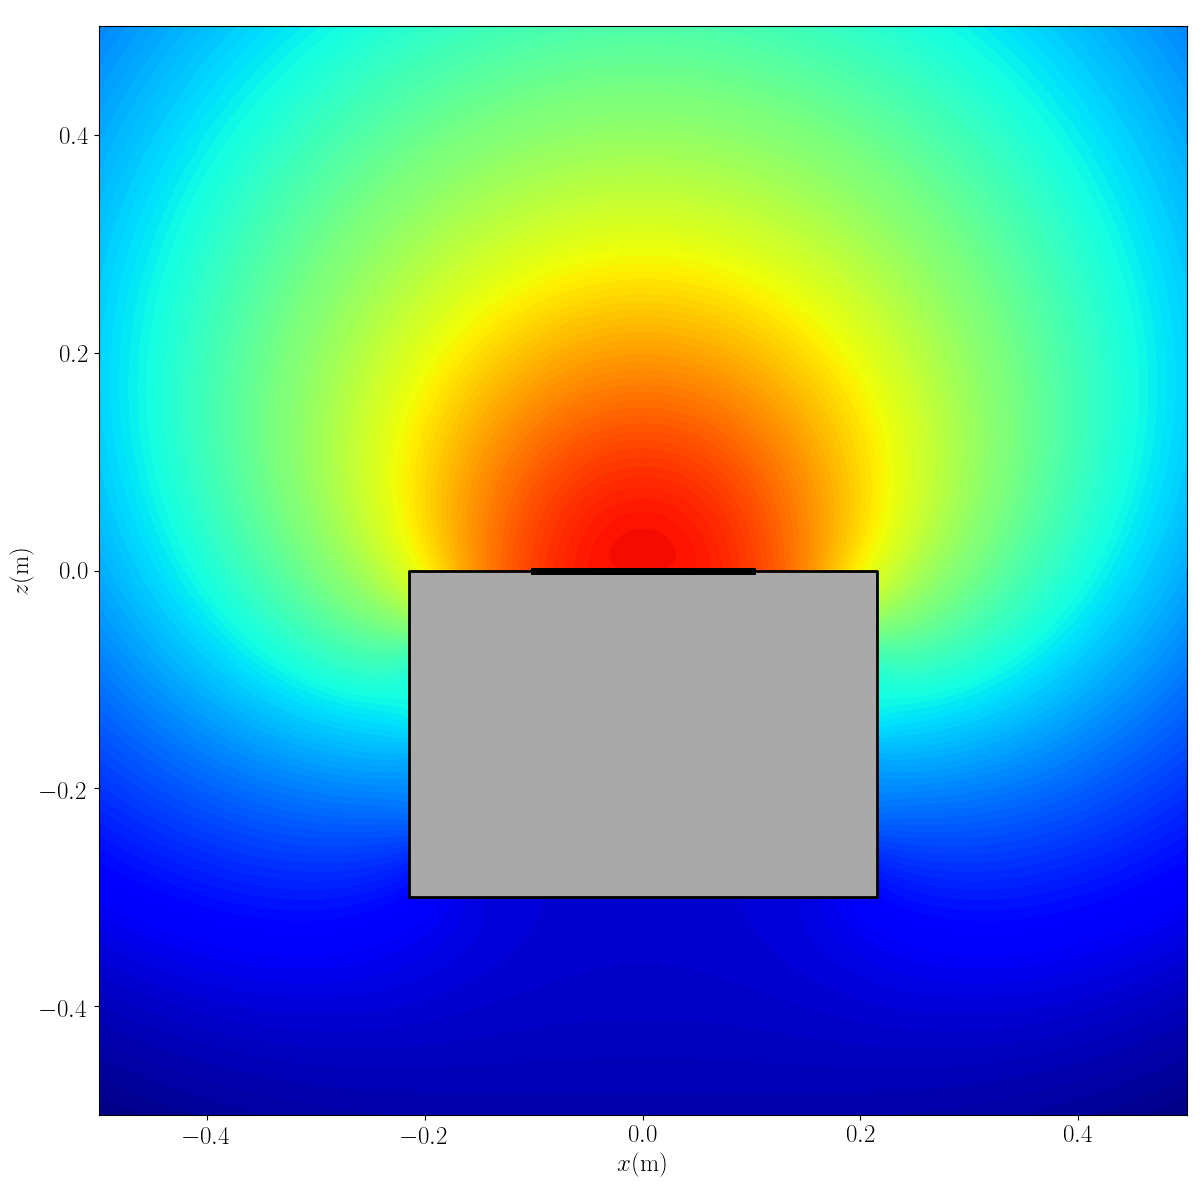
\includegraphics[width=3in]{figures/100.png}}%
    \only<2>{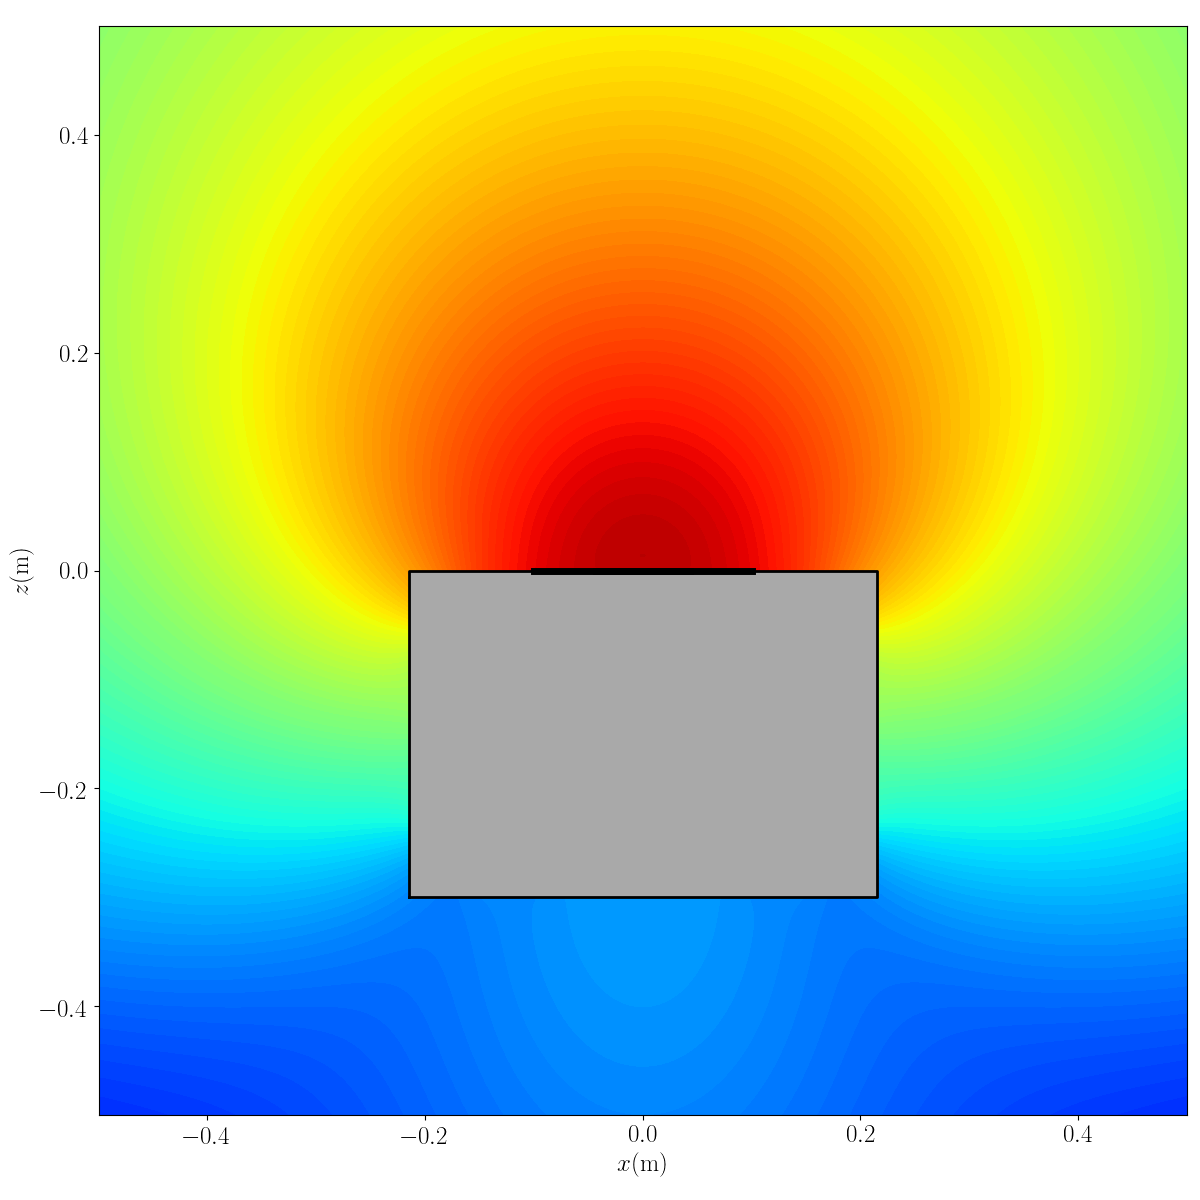
\includegraphics[width=3in]{figures/200.png}}%
    \only<3>{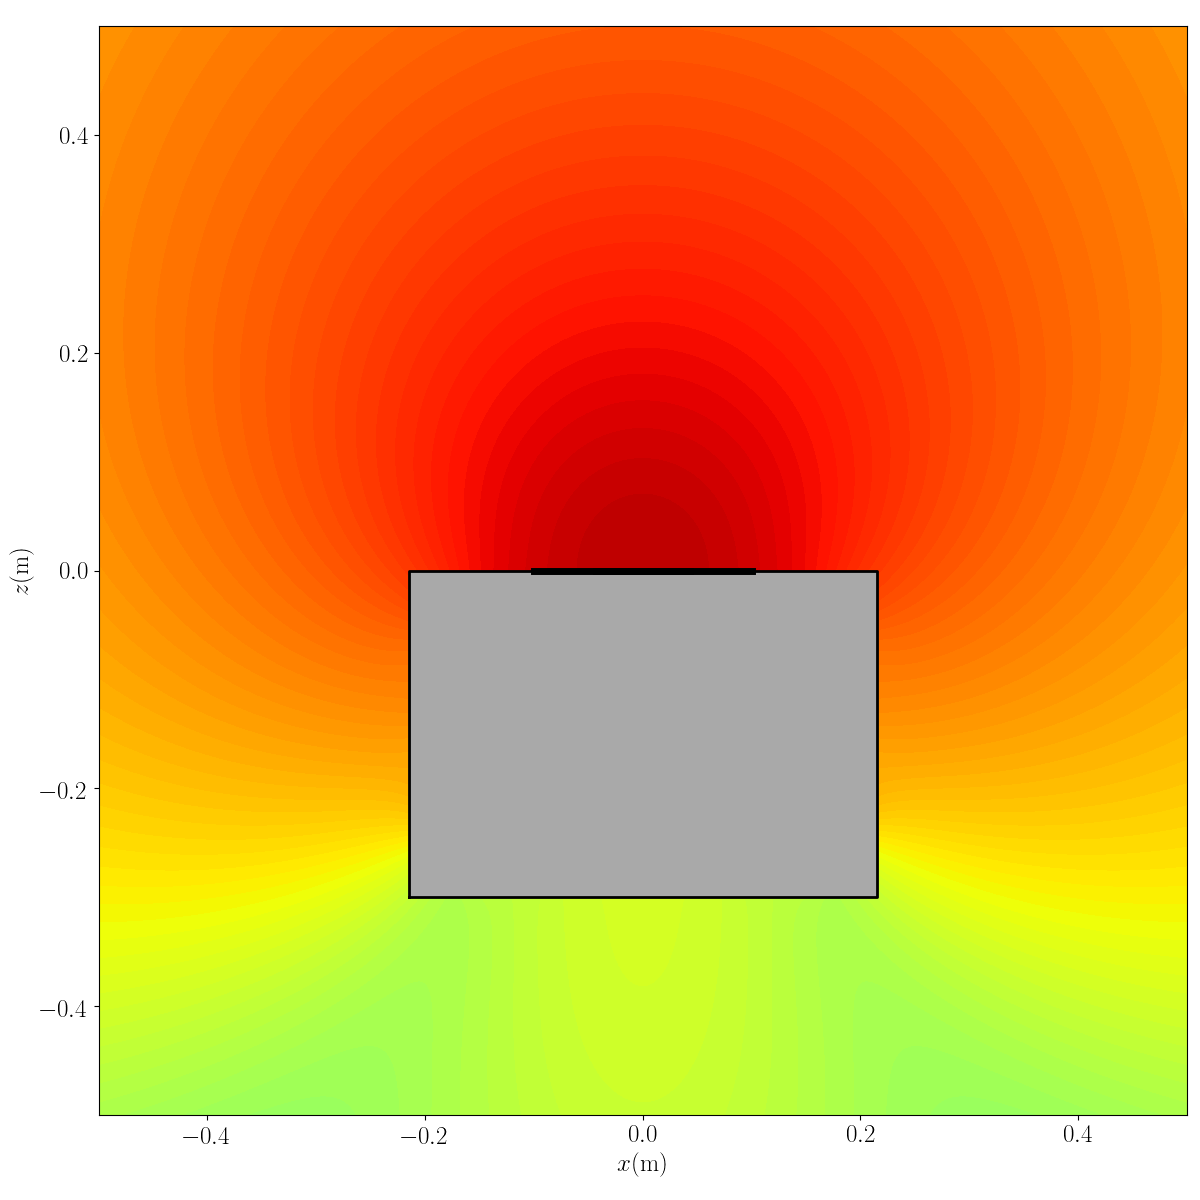
\includegraphics[width=3in]{figures/300.png}}%
    \only<4>{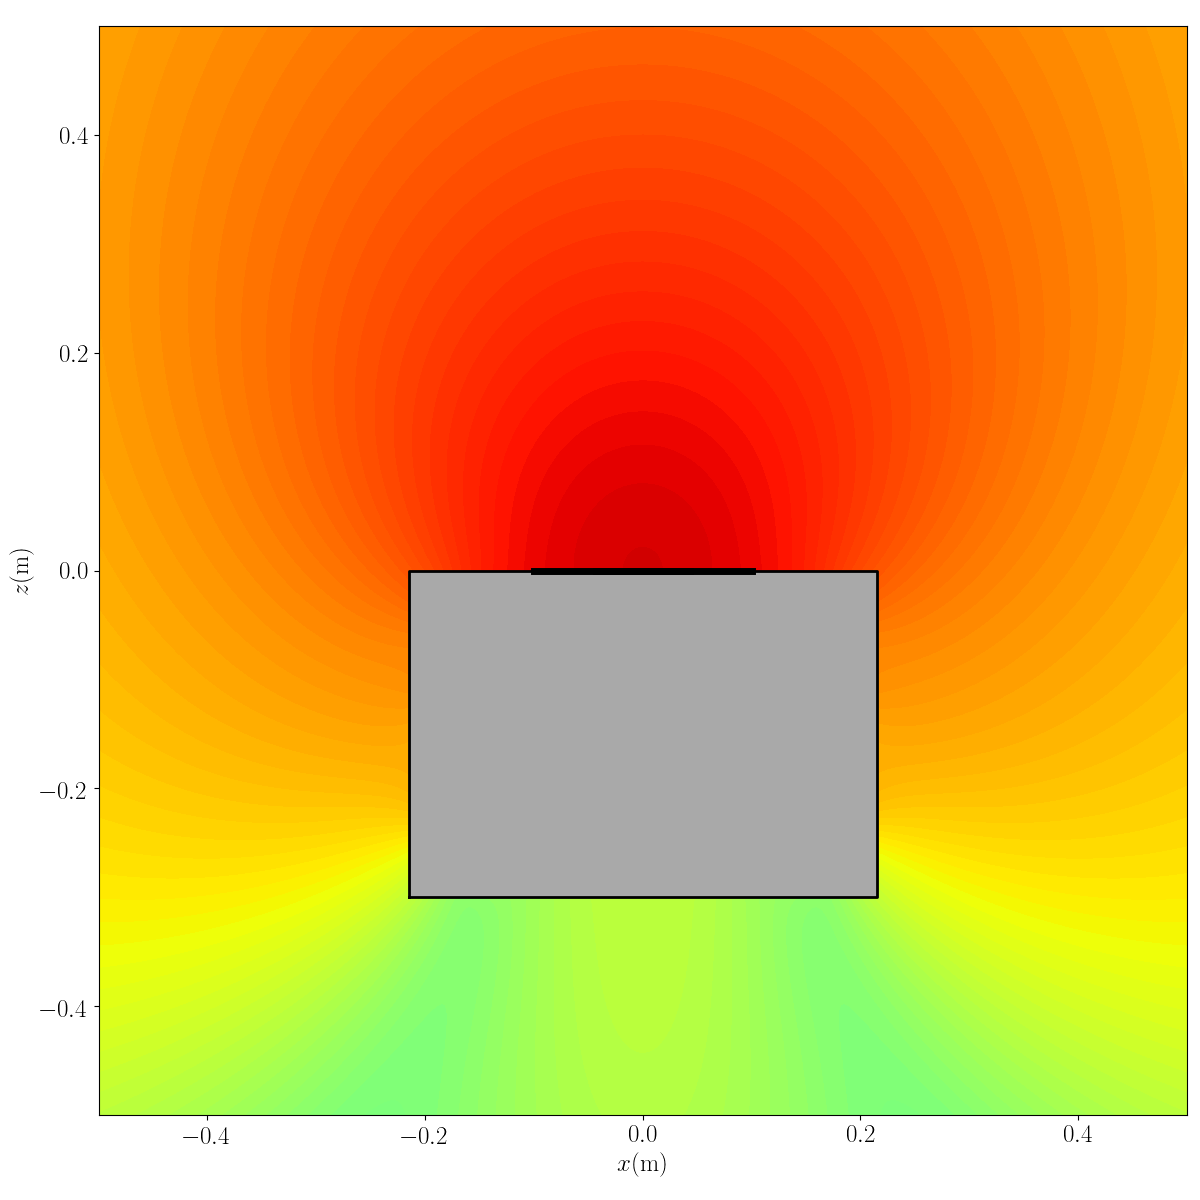
\includegraphics[width=3in]{figures/400.png}}%
    \only<5>{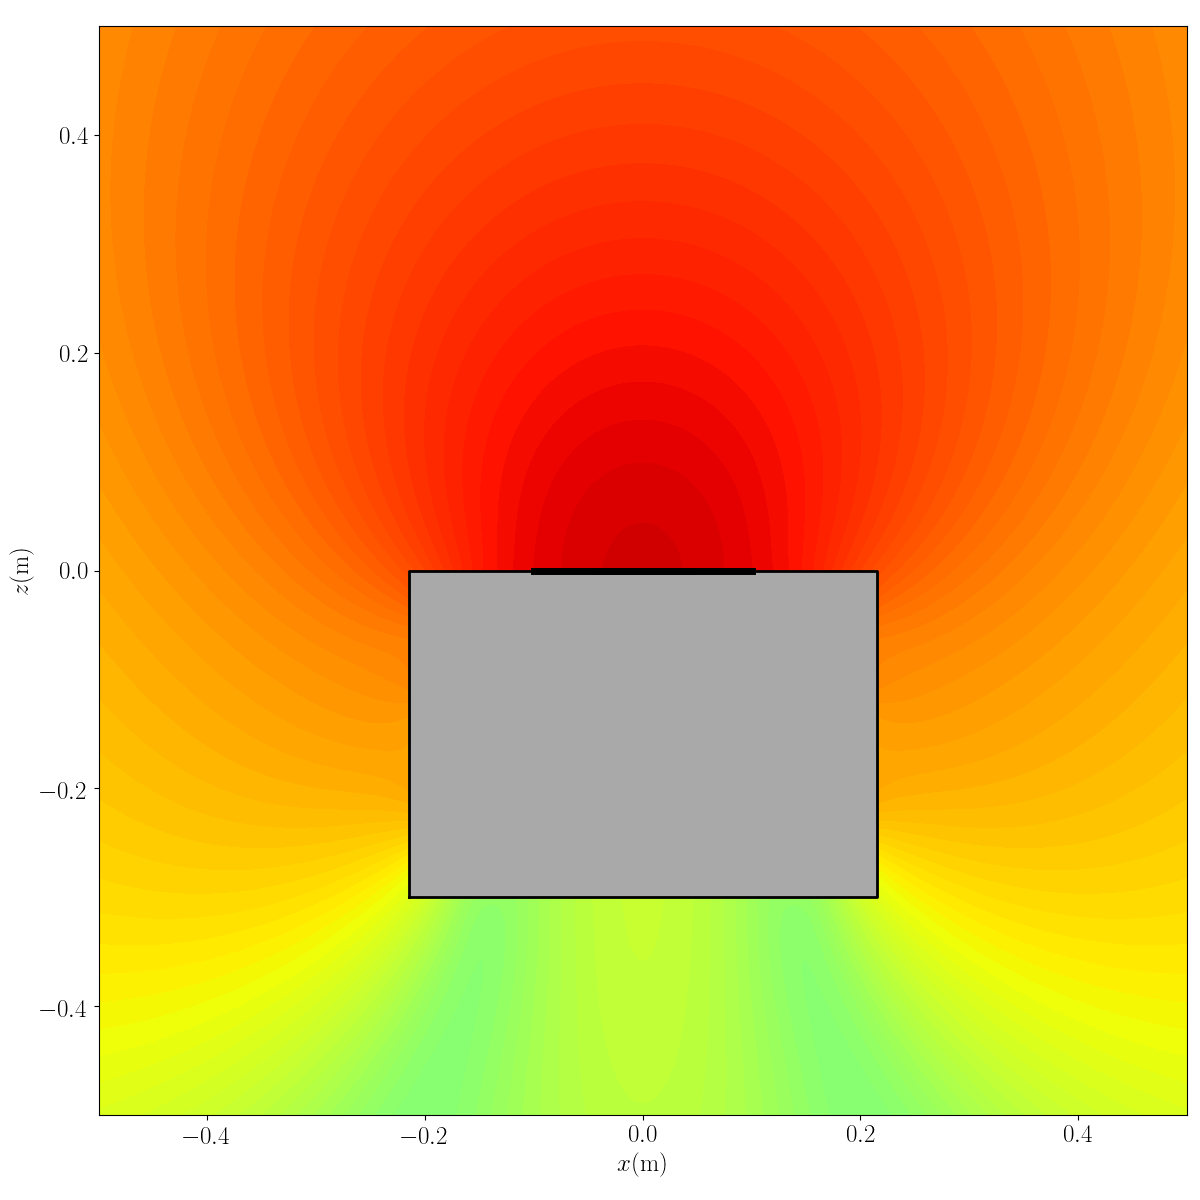
\includegraphics[width=3in]{figures/500.png}}%
    \only<6>{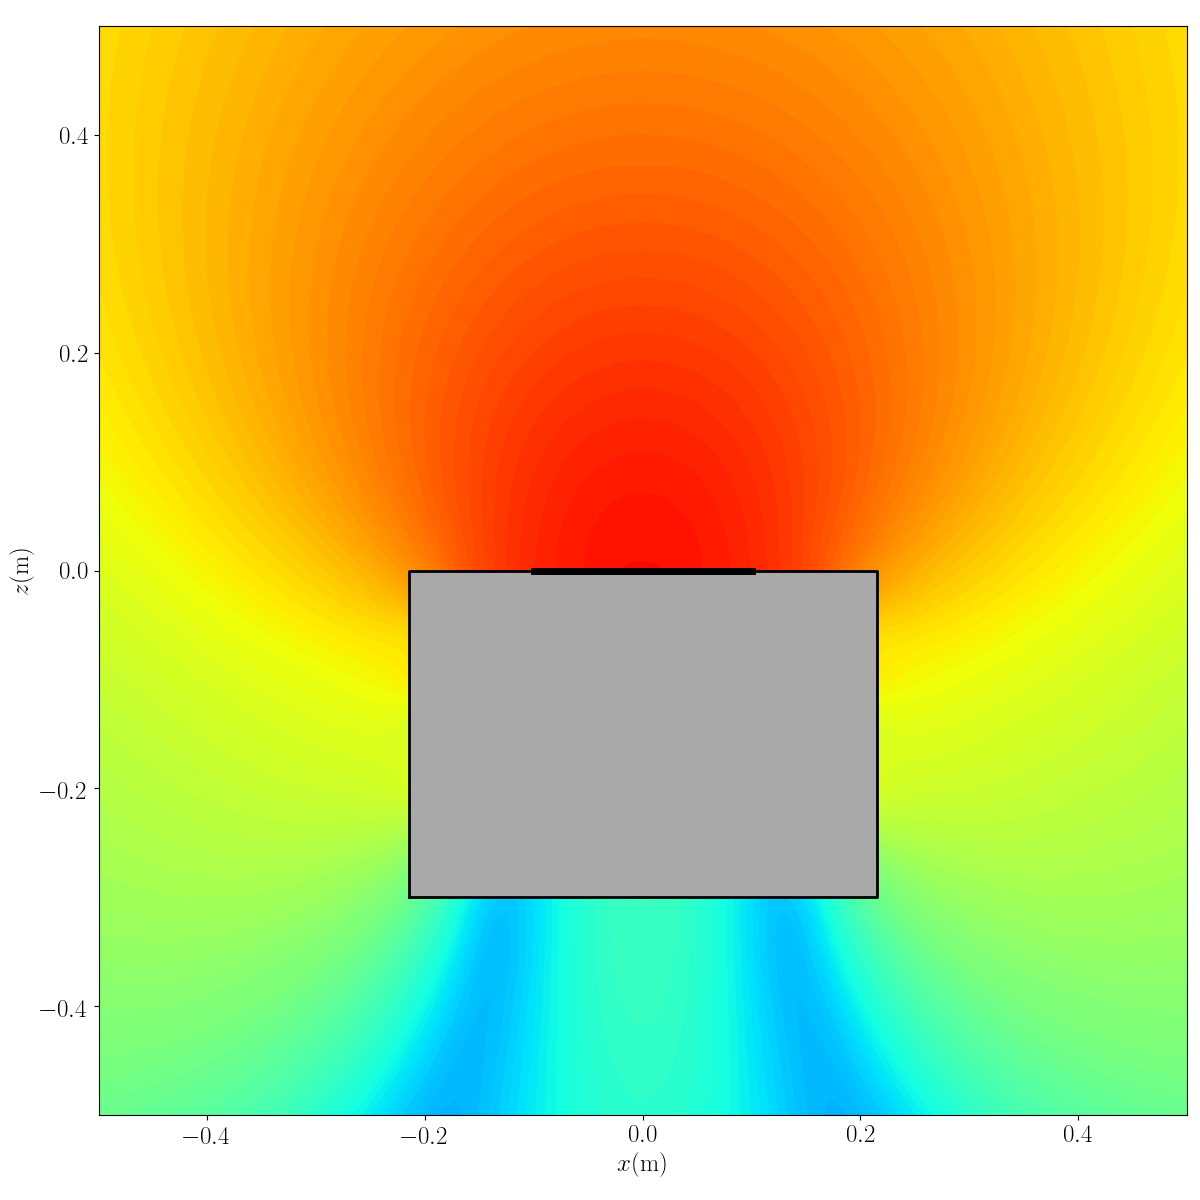
\includegraphics[width=3in]{figures/600.png}}%
    \only<7>{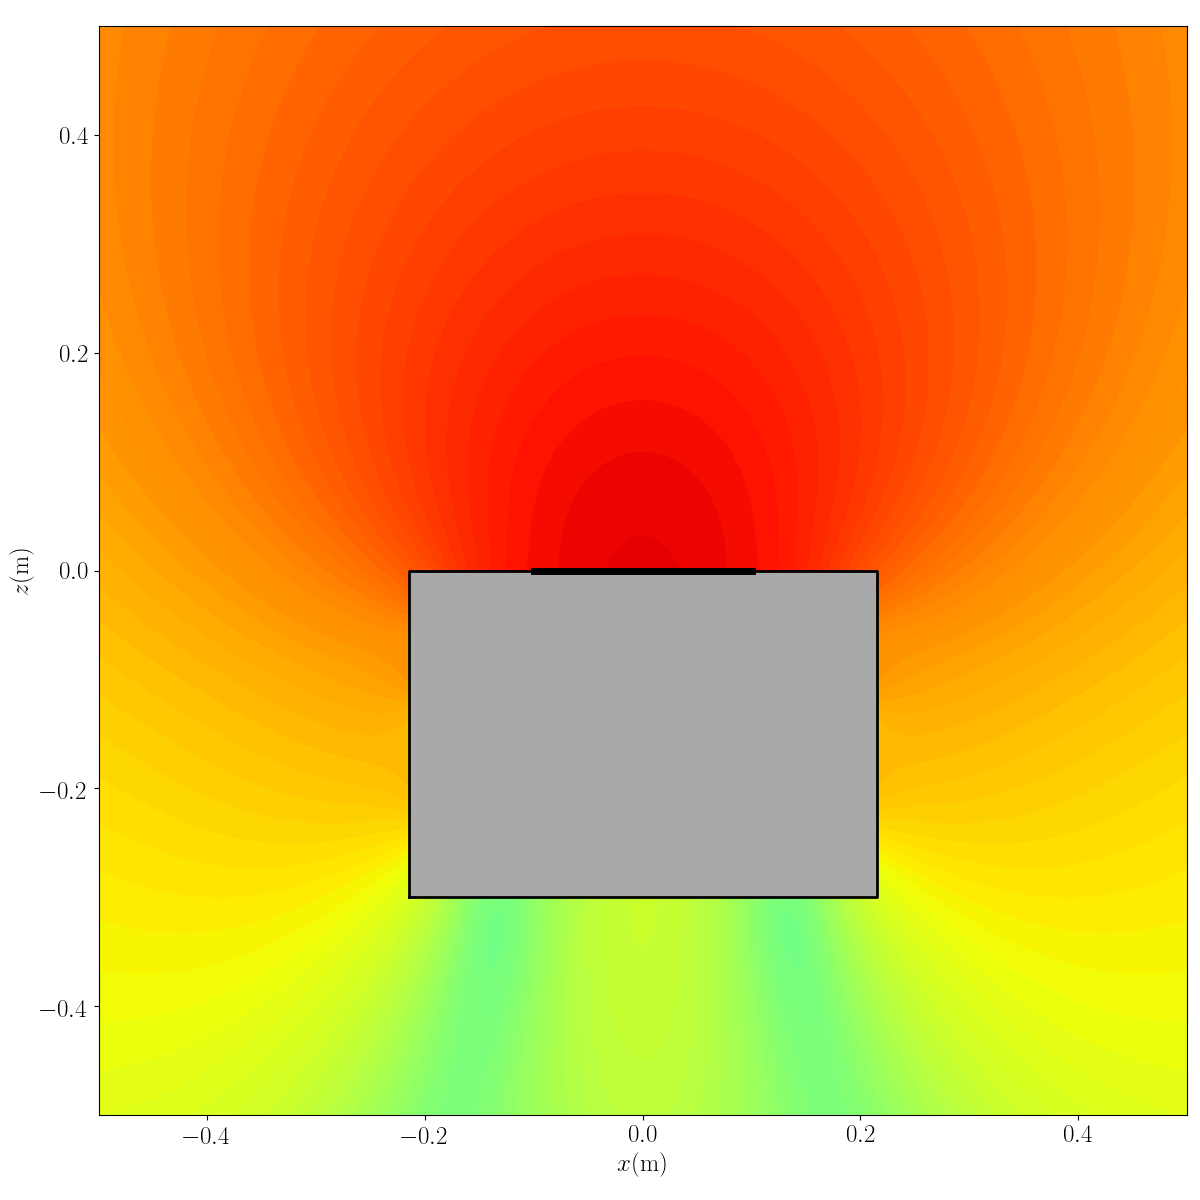
\includegraphics[width=3in]{figures/700.png}}%
    \only<8>{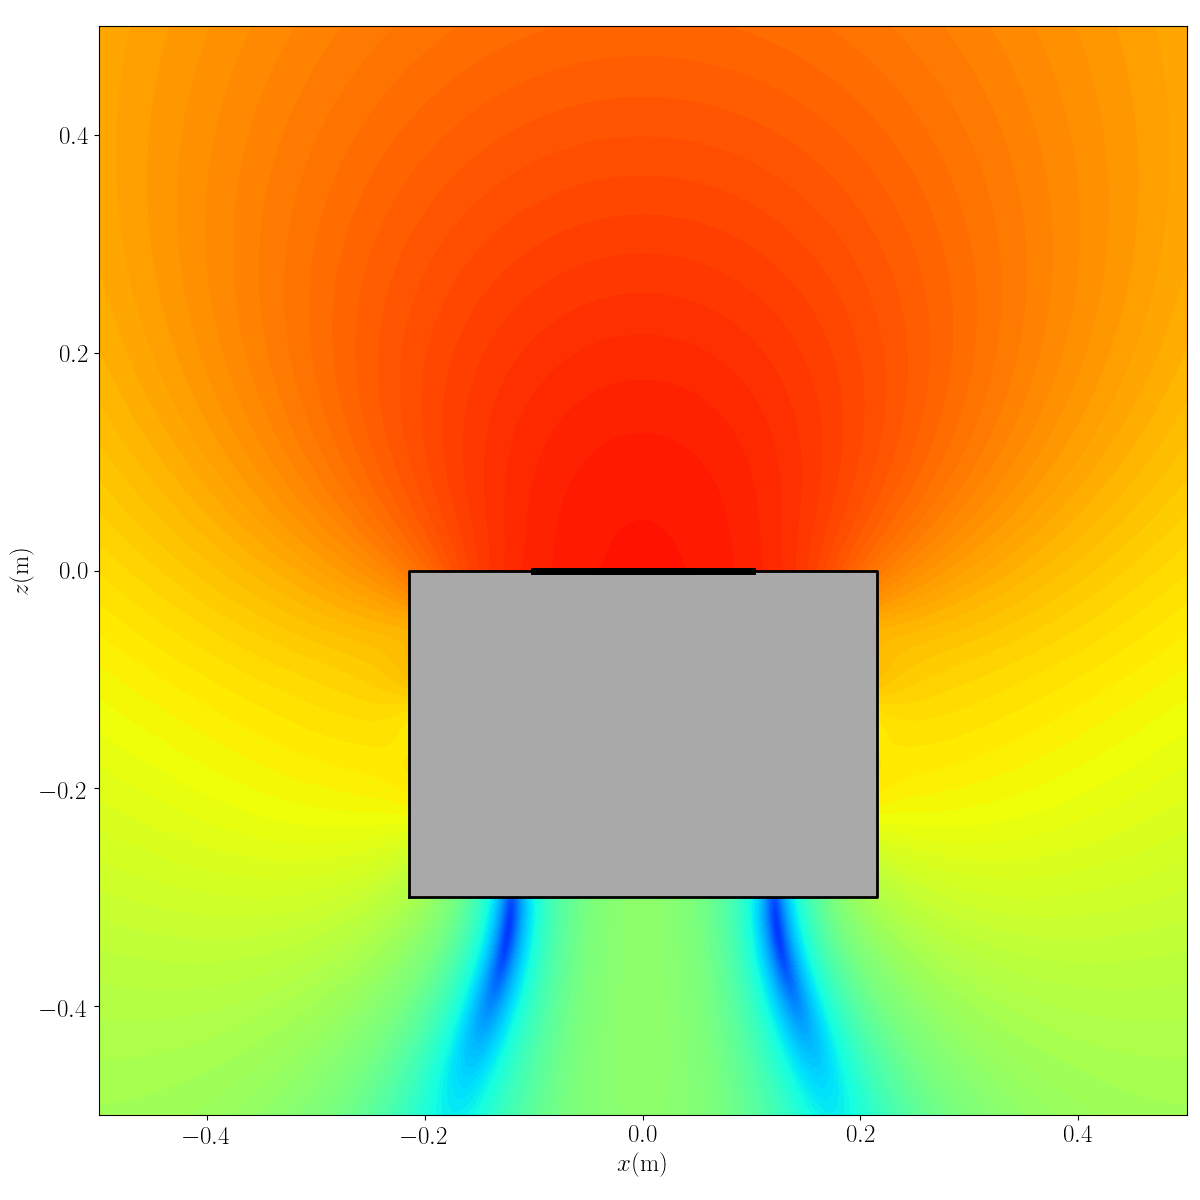
\includegraphics[width=3in]{figures/800.png}}%
    \only<9>{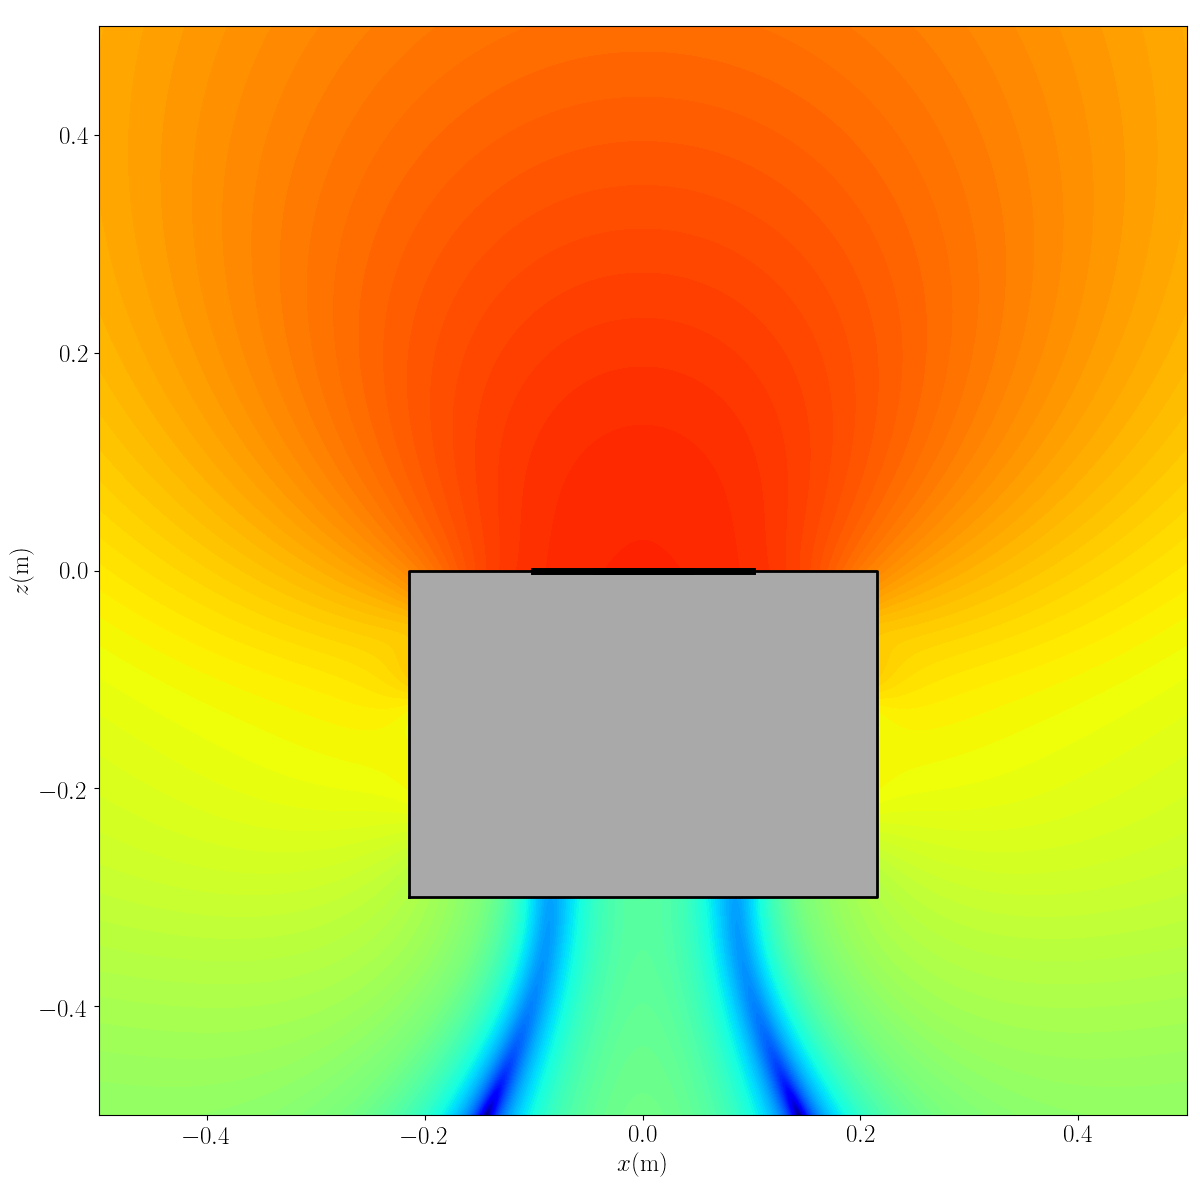
\includegraphics[width=3in]{figures/900.png}}%
    \only<10>{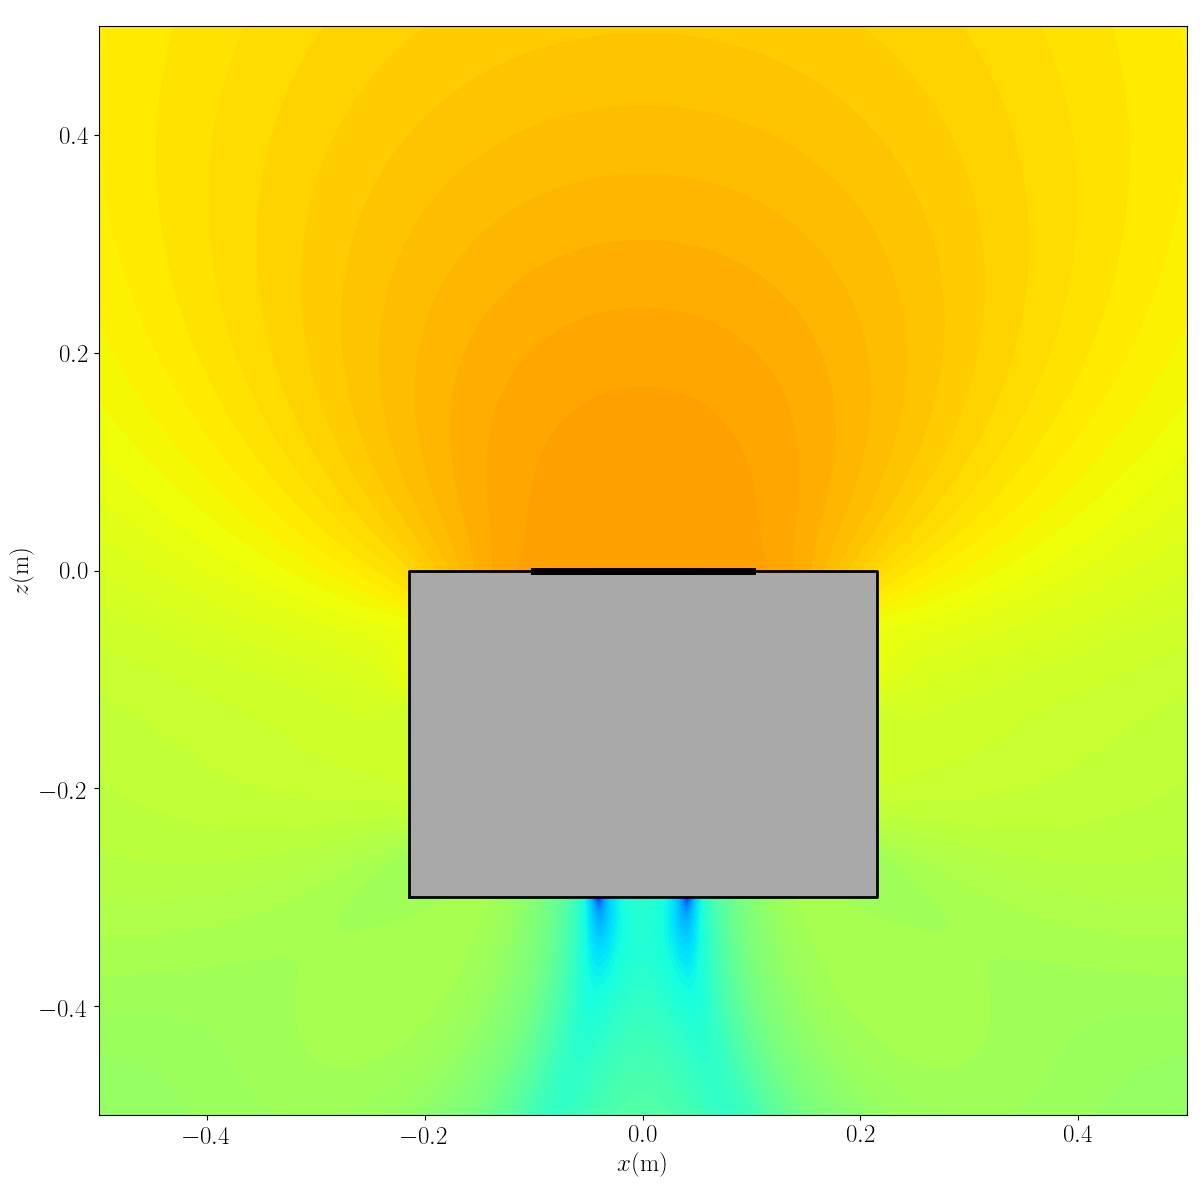
\includegraphics[width=3in]{figures/1000.png}}%
    \only<11>{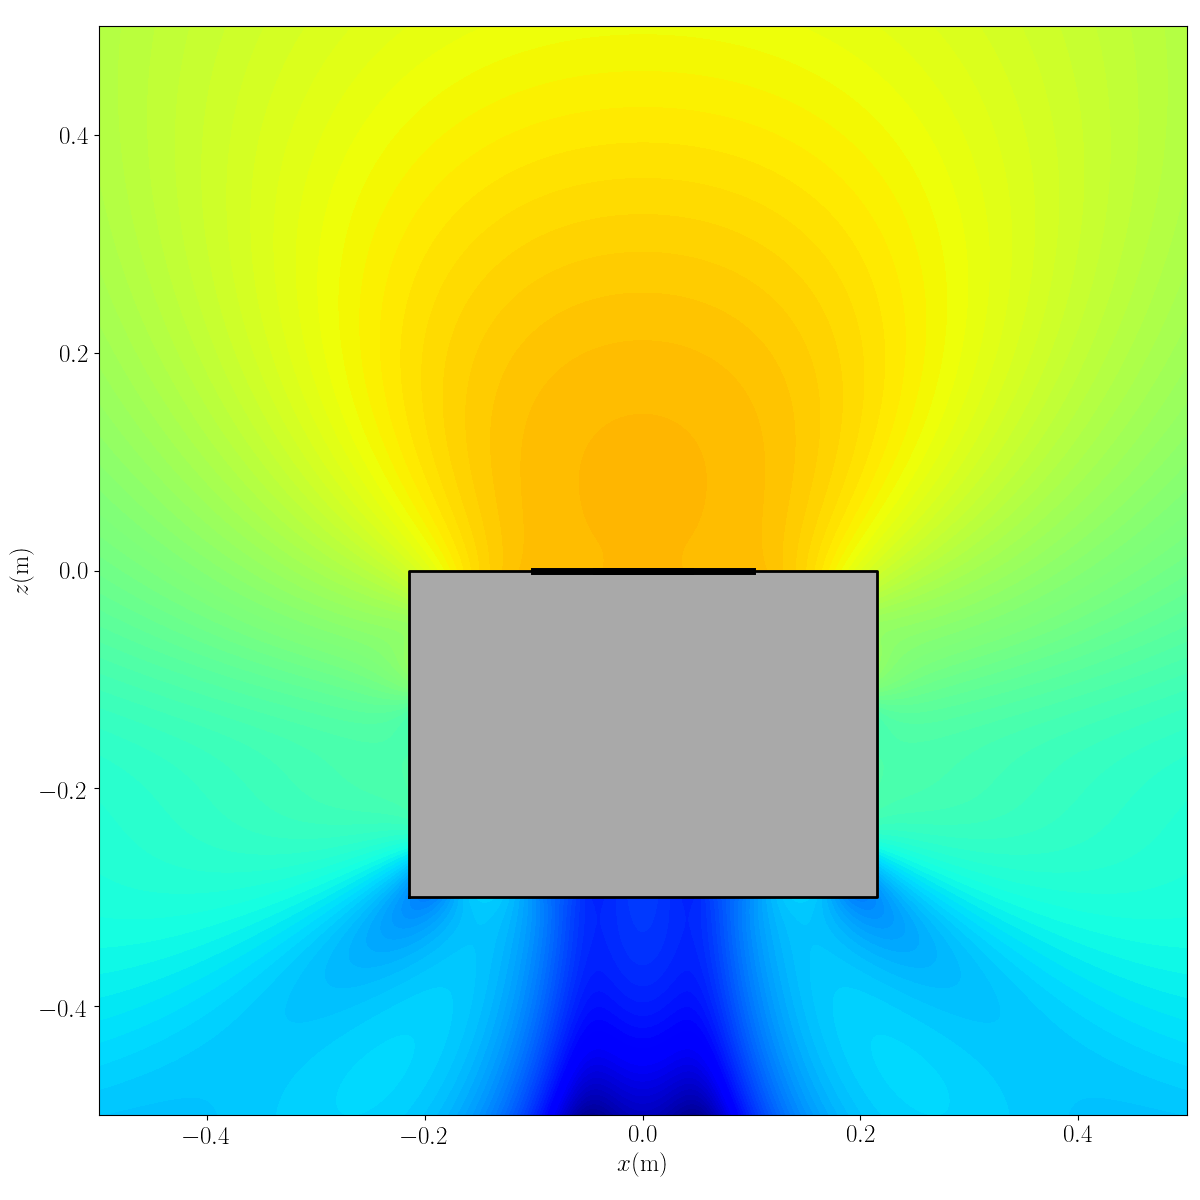
\includegraphics[width=3in]{figures/1100.png}}%
    \only<12>{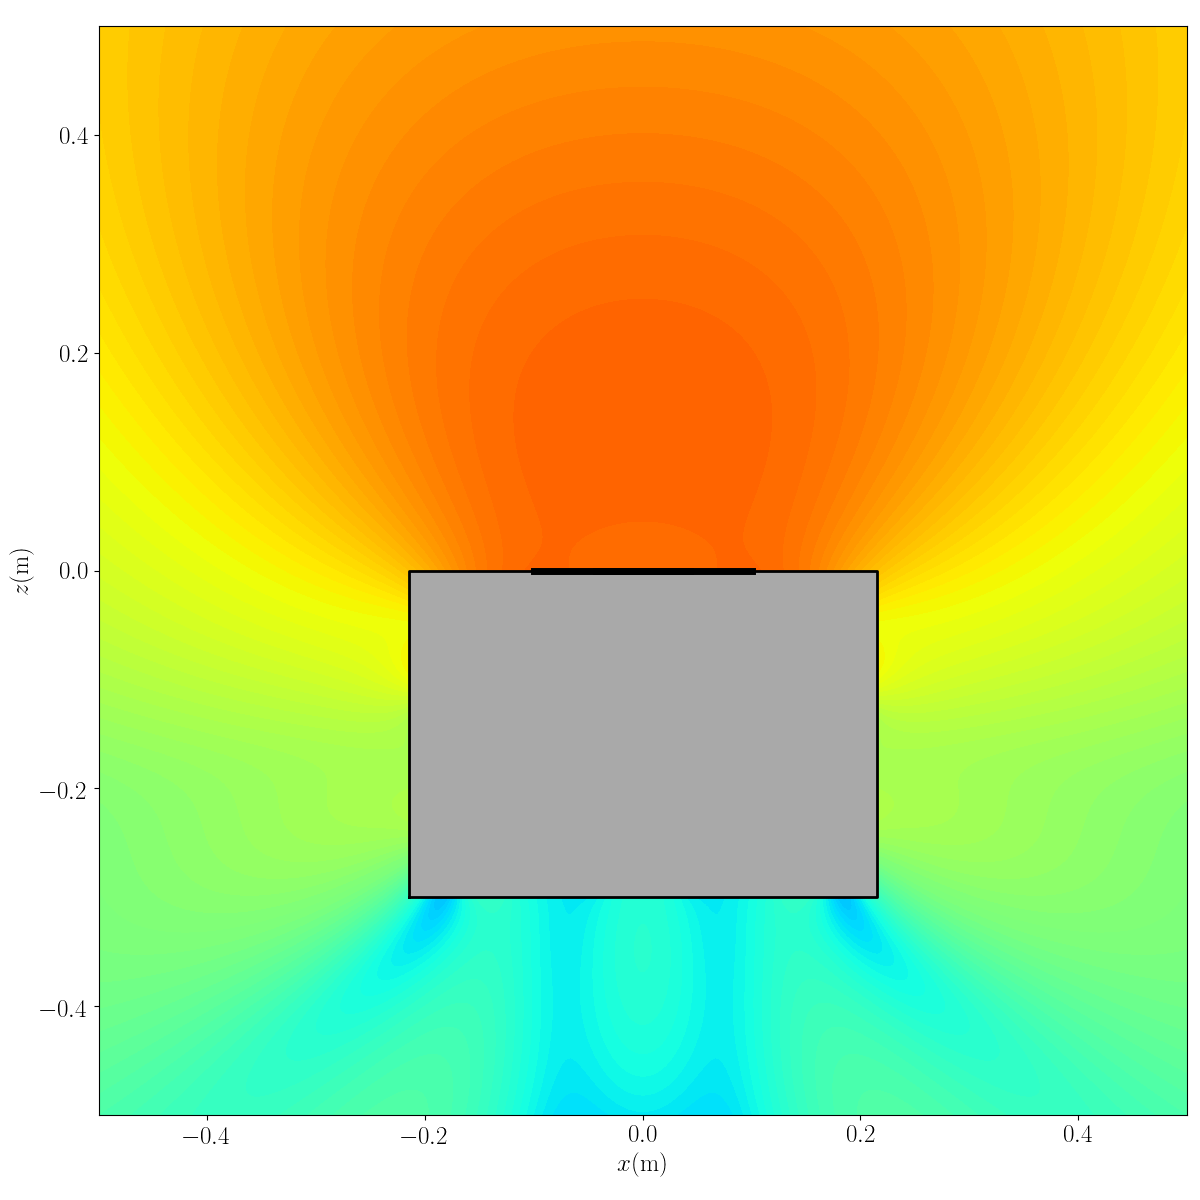
\includegraphics[width=3in]{figures/1200.png}}%
    \only<13>{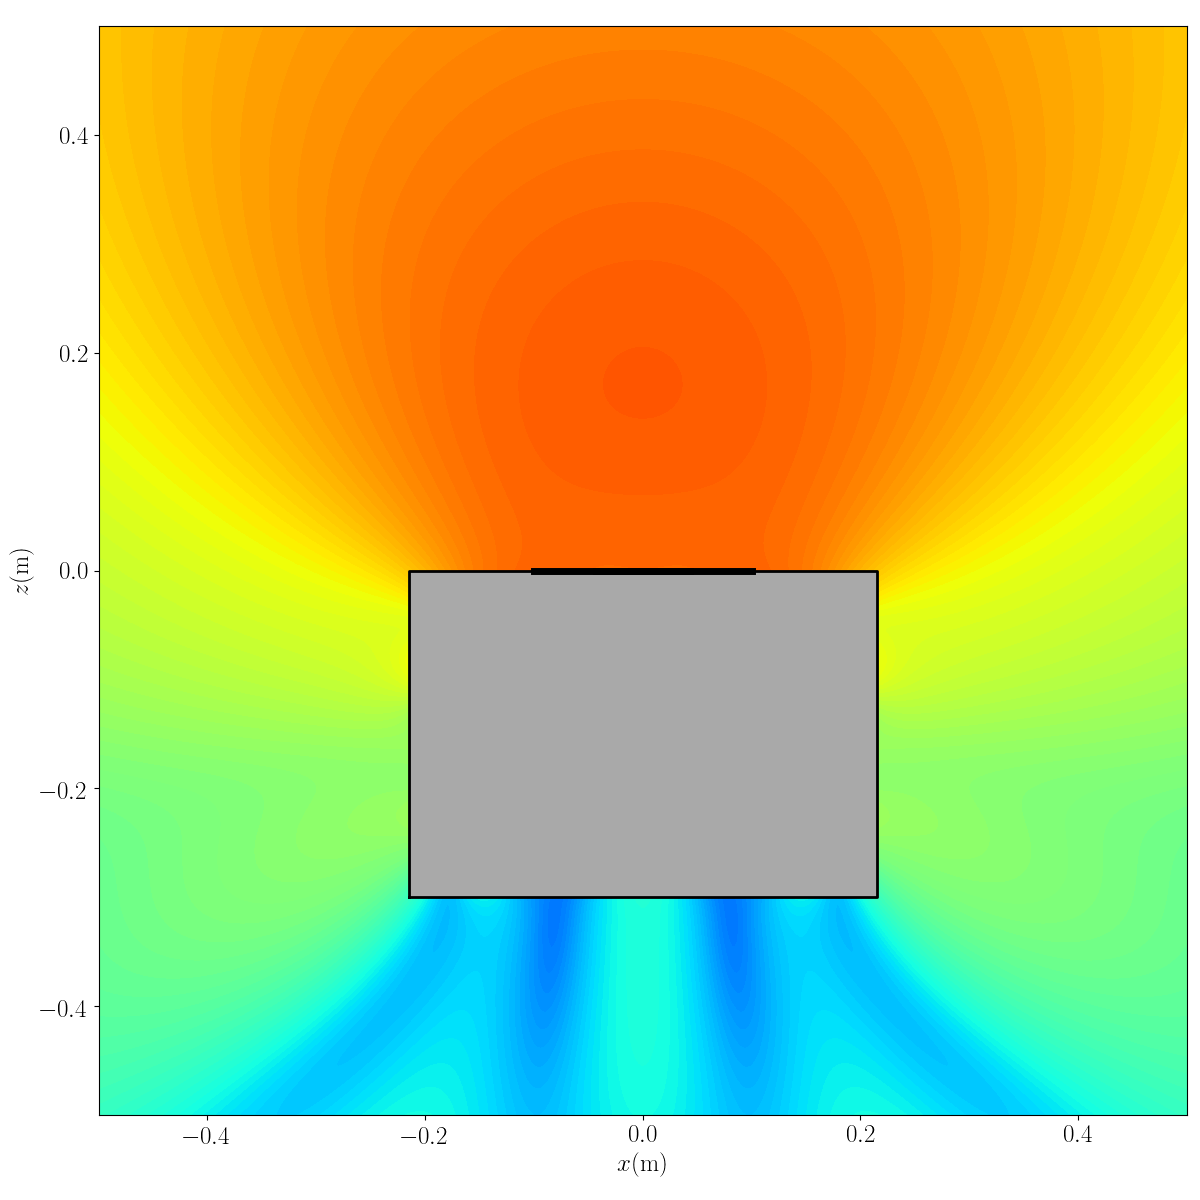
\includegraphics[width=3in]{figures/1300.png}}%
    \only<14>{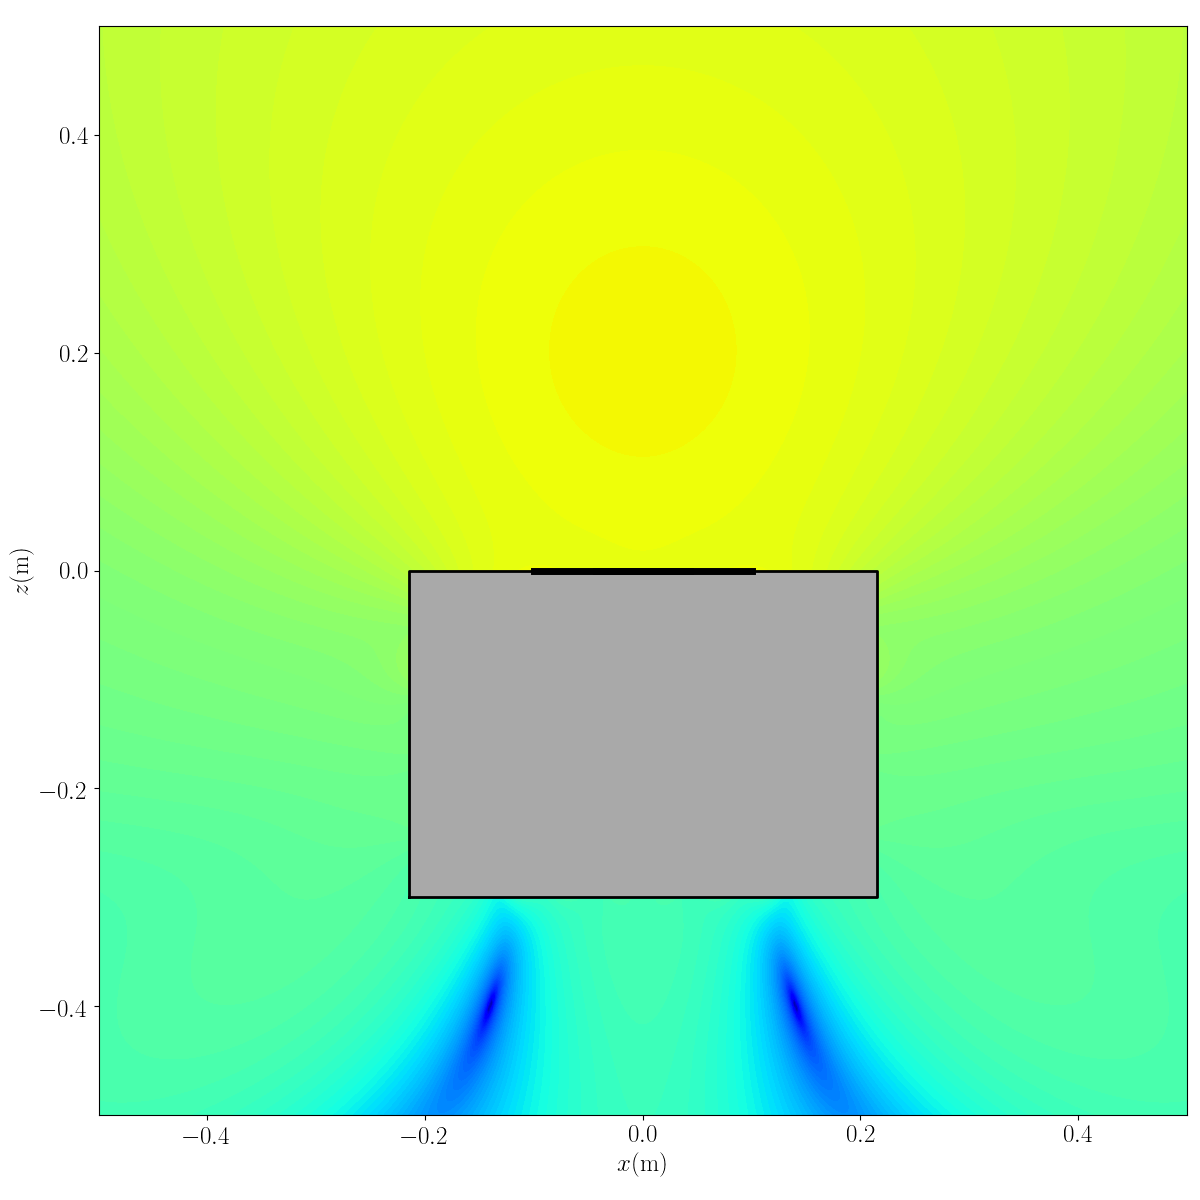
\includegraphics[width=3in]{figures/1400.png}}%
    \only<15>{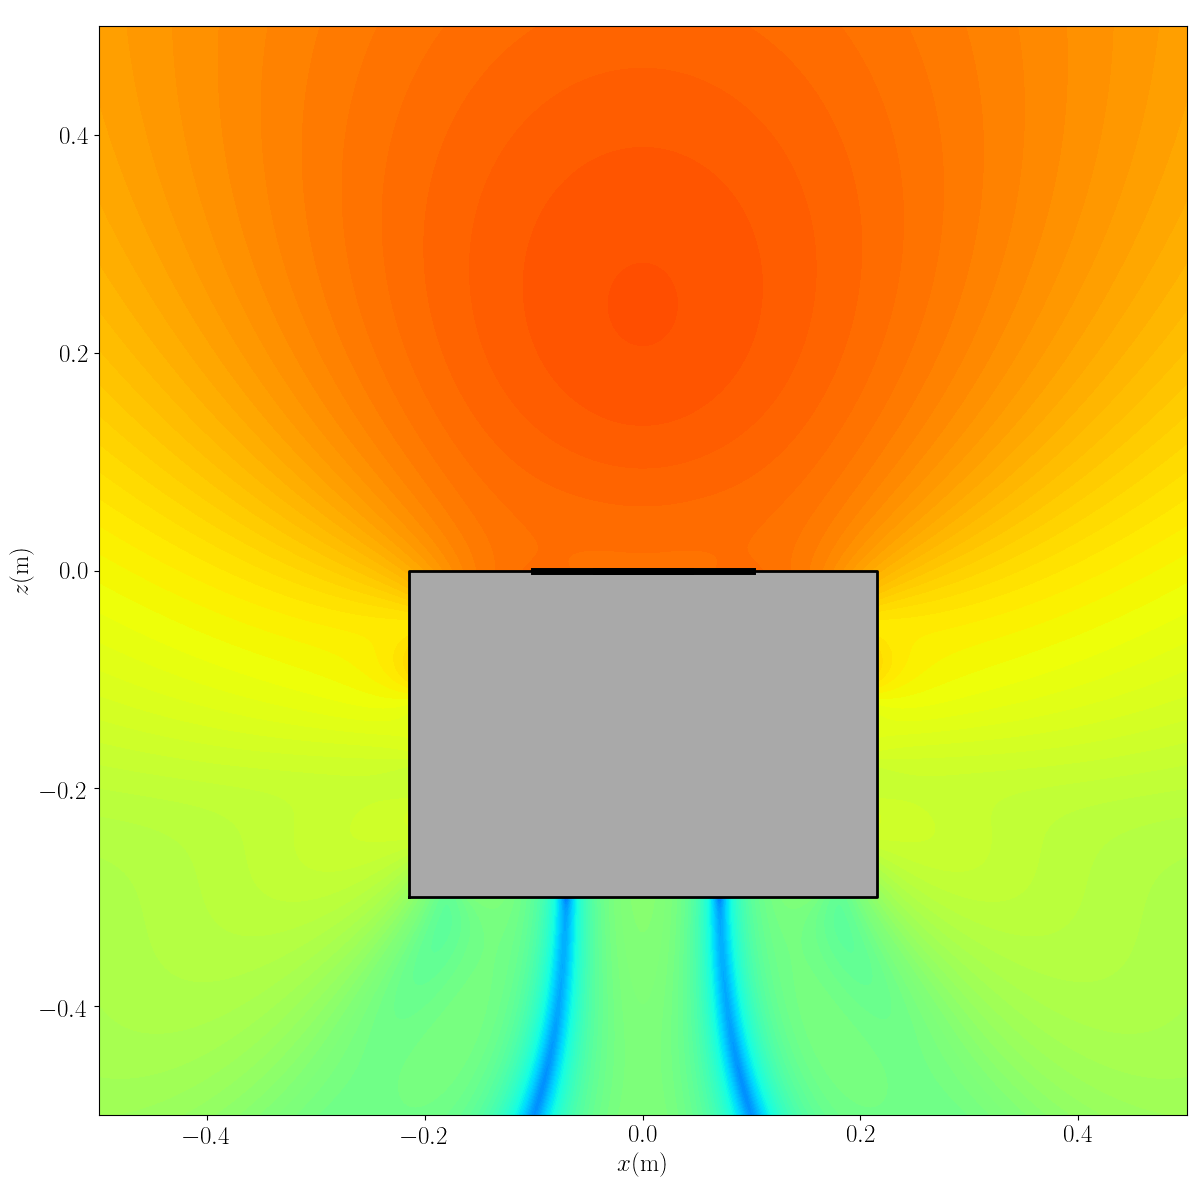
\includegraphics[width=3in]{figures/1500.png}}%
    \only<16>{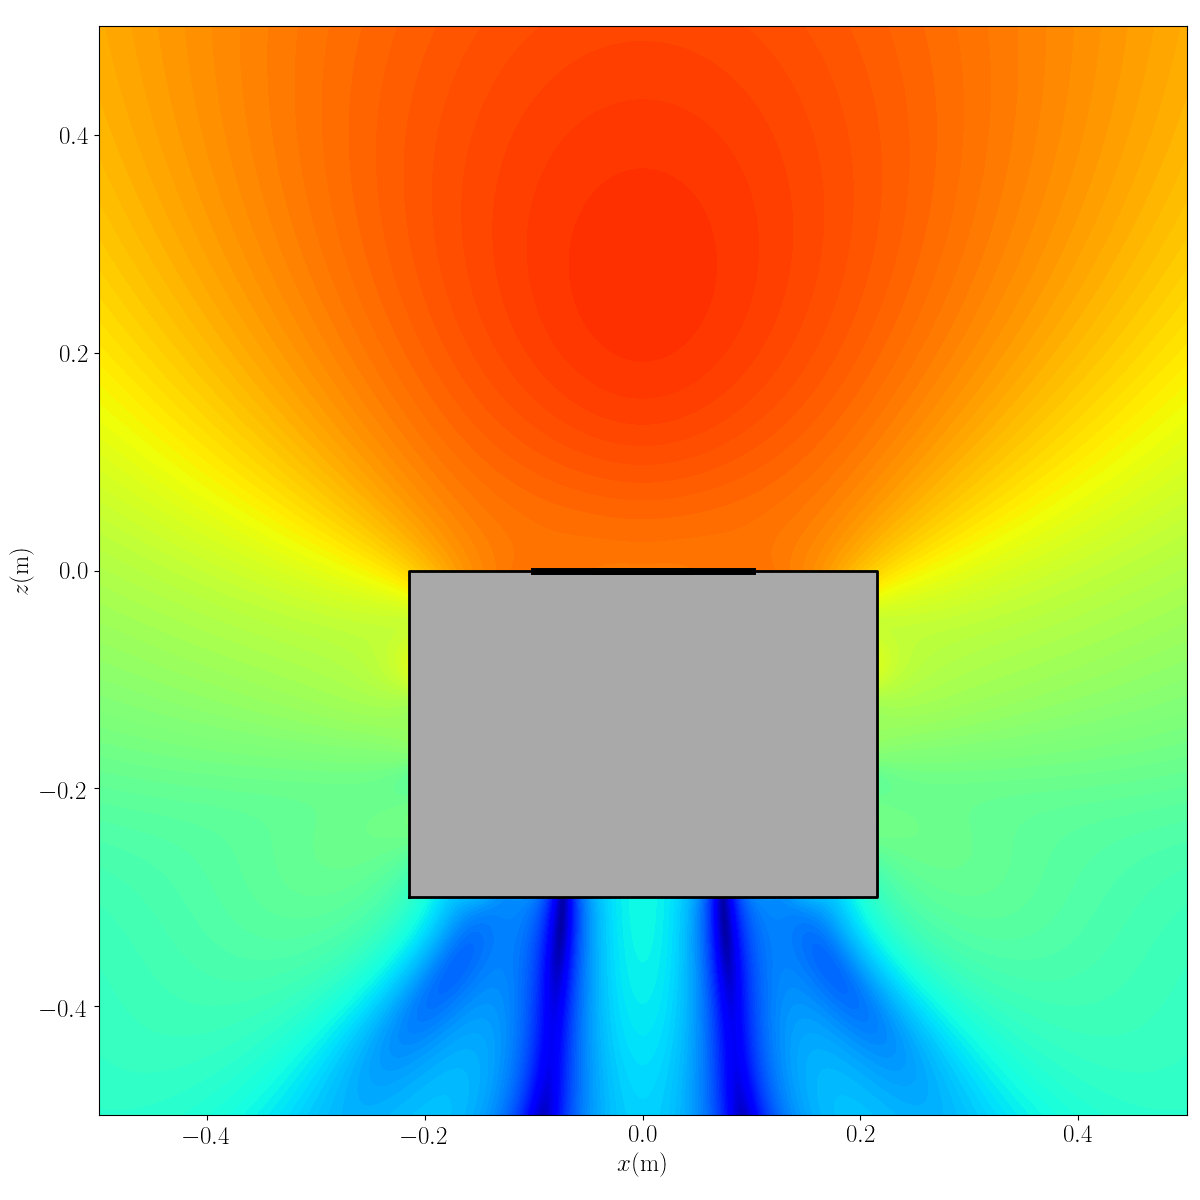
\includegraphics[width=3in]{figures/1600.png}}%
    \only<17>{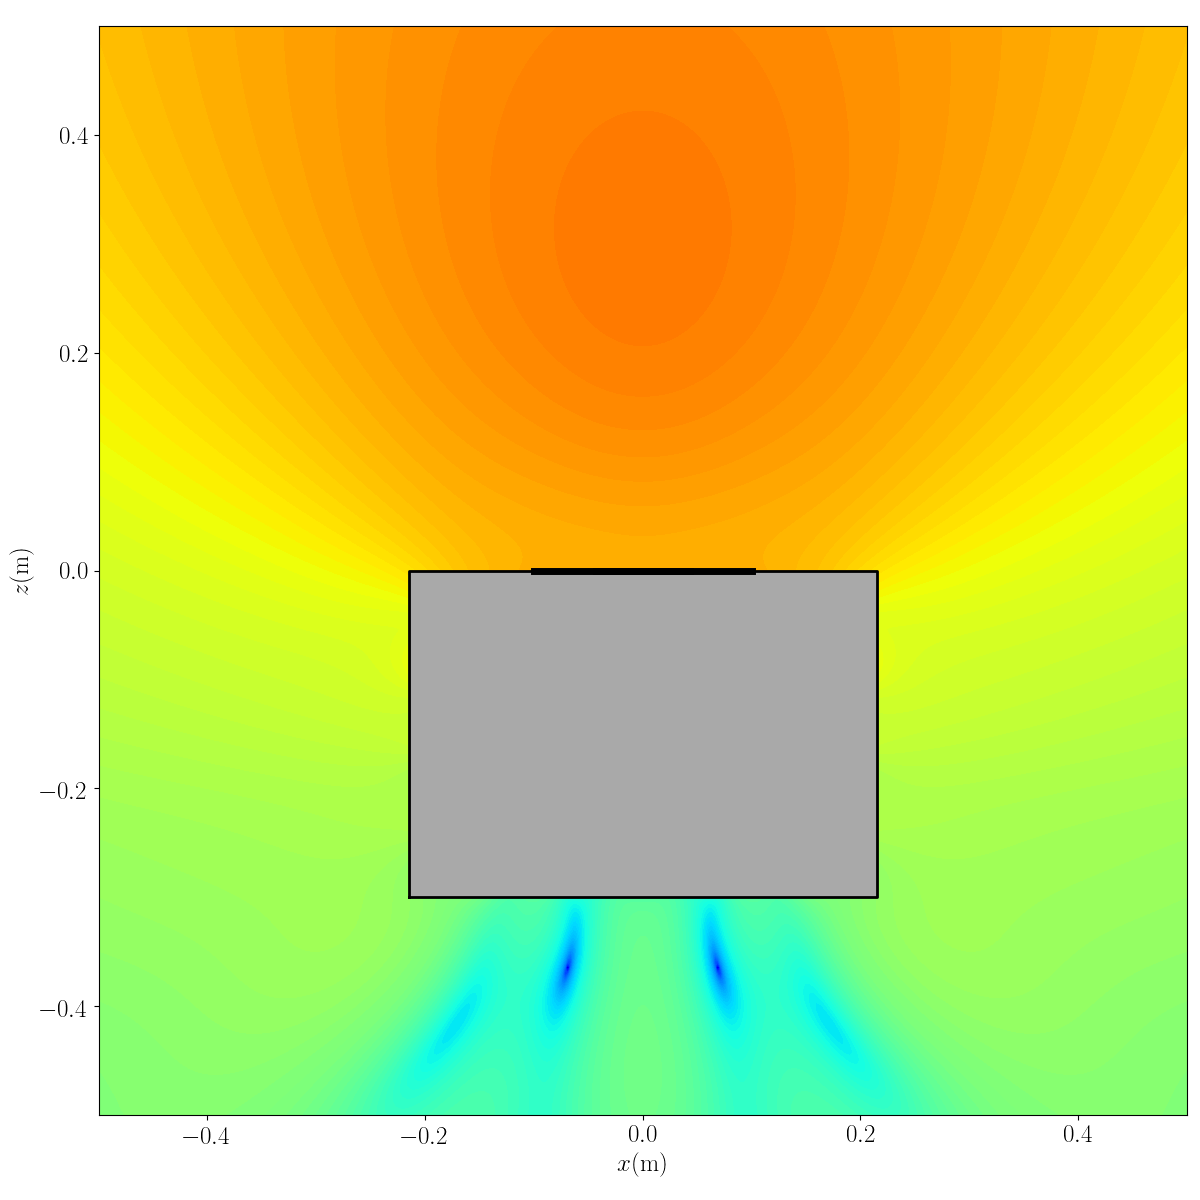
\includegraphics[width=3in]{figures/1700.png}}%
    \only<18>{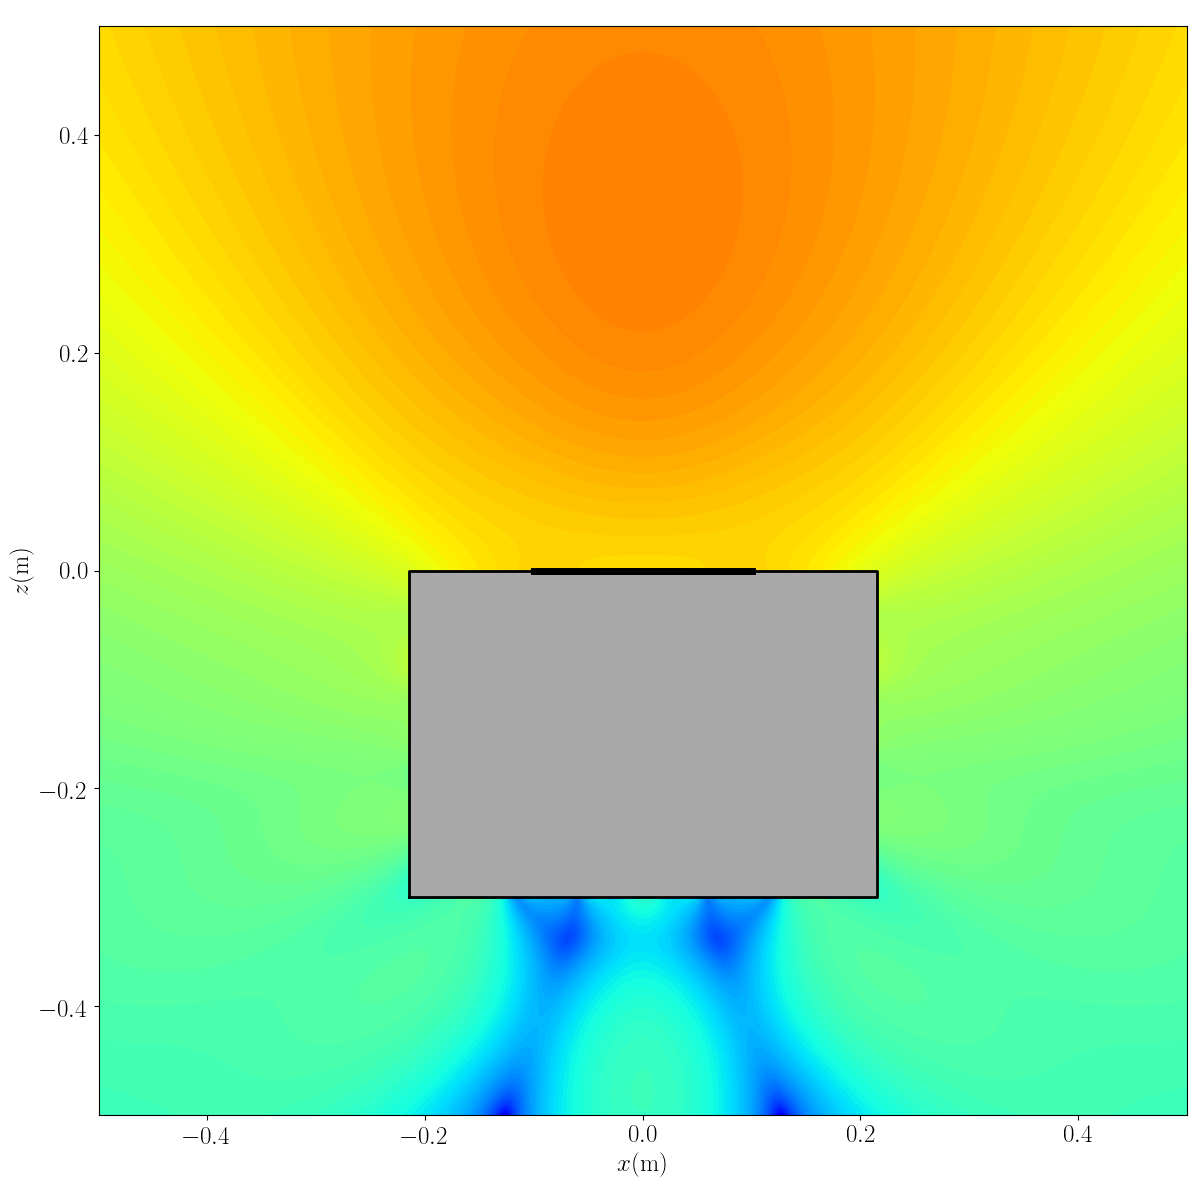
\includegraphics[width=3in]{figures/1800.png}}%
    \only<19>{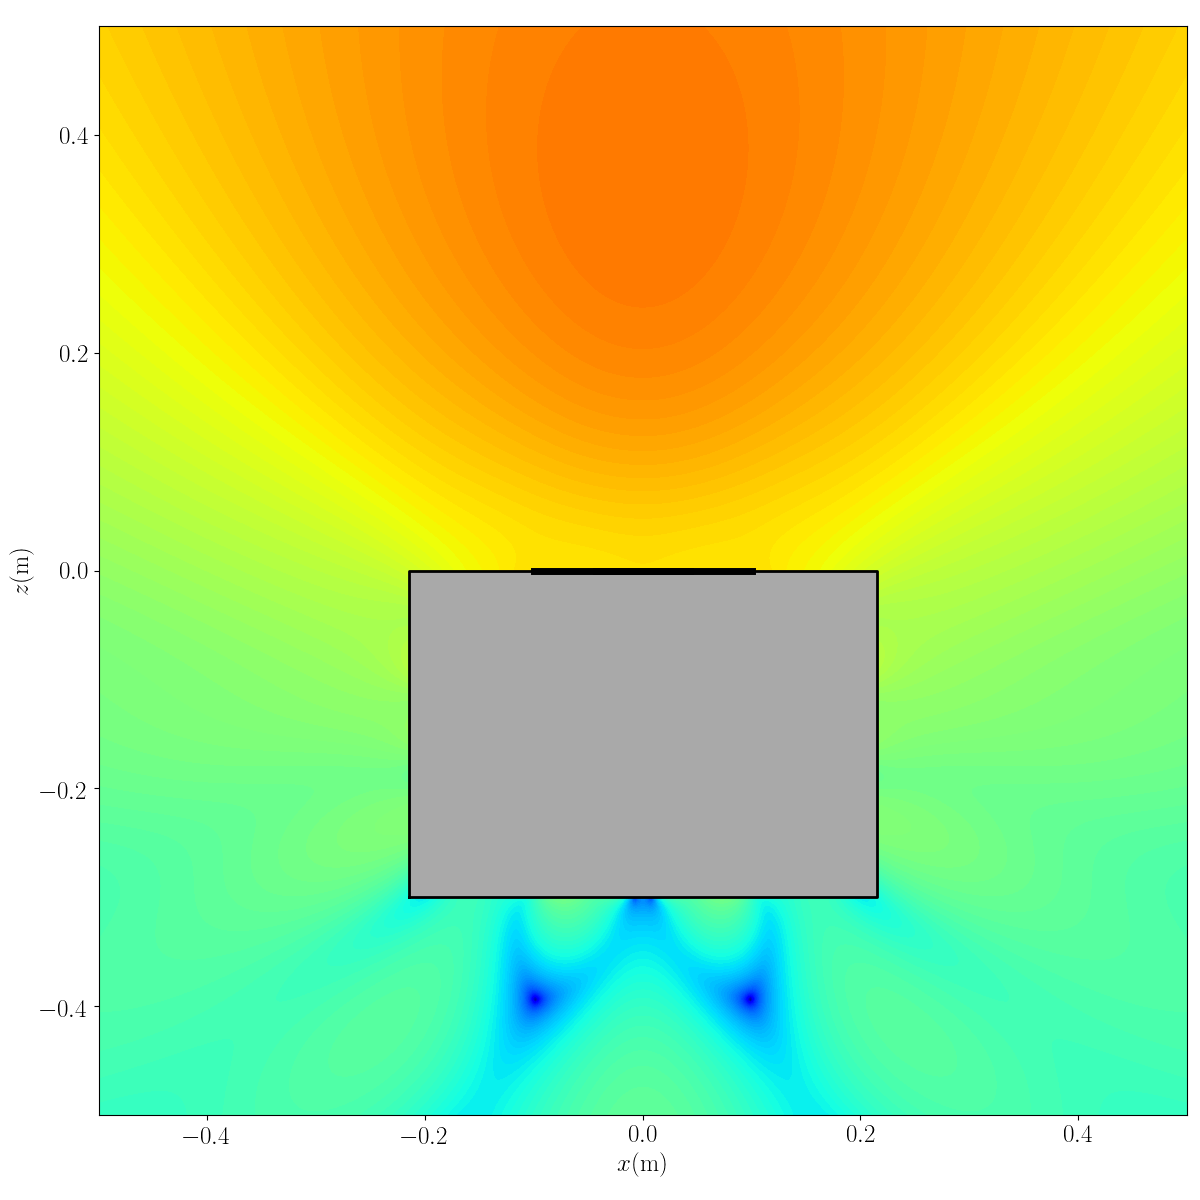
\includegraphics[width=3in]{figures/1900.png}}%
    \only<20>{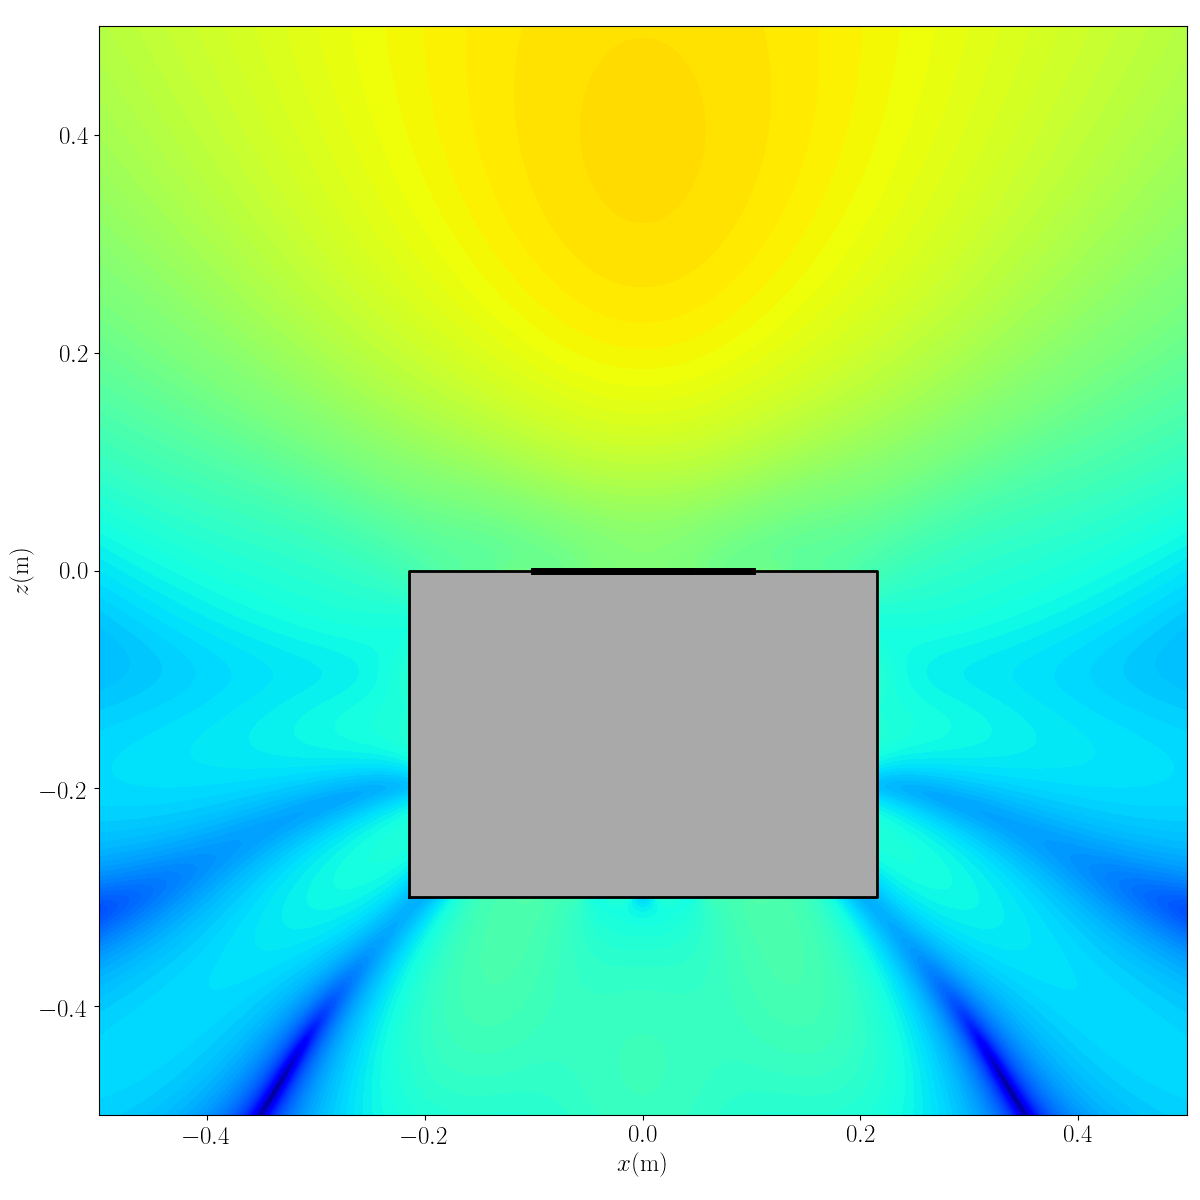
\includegraphics[width=3in]{figures/2000.png}}%
    \only<21>{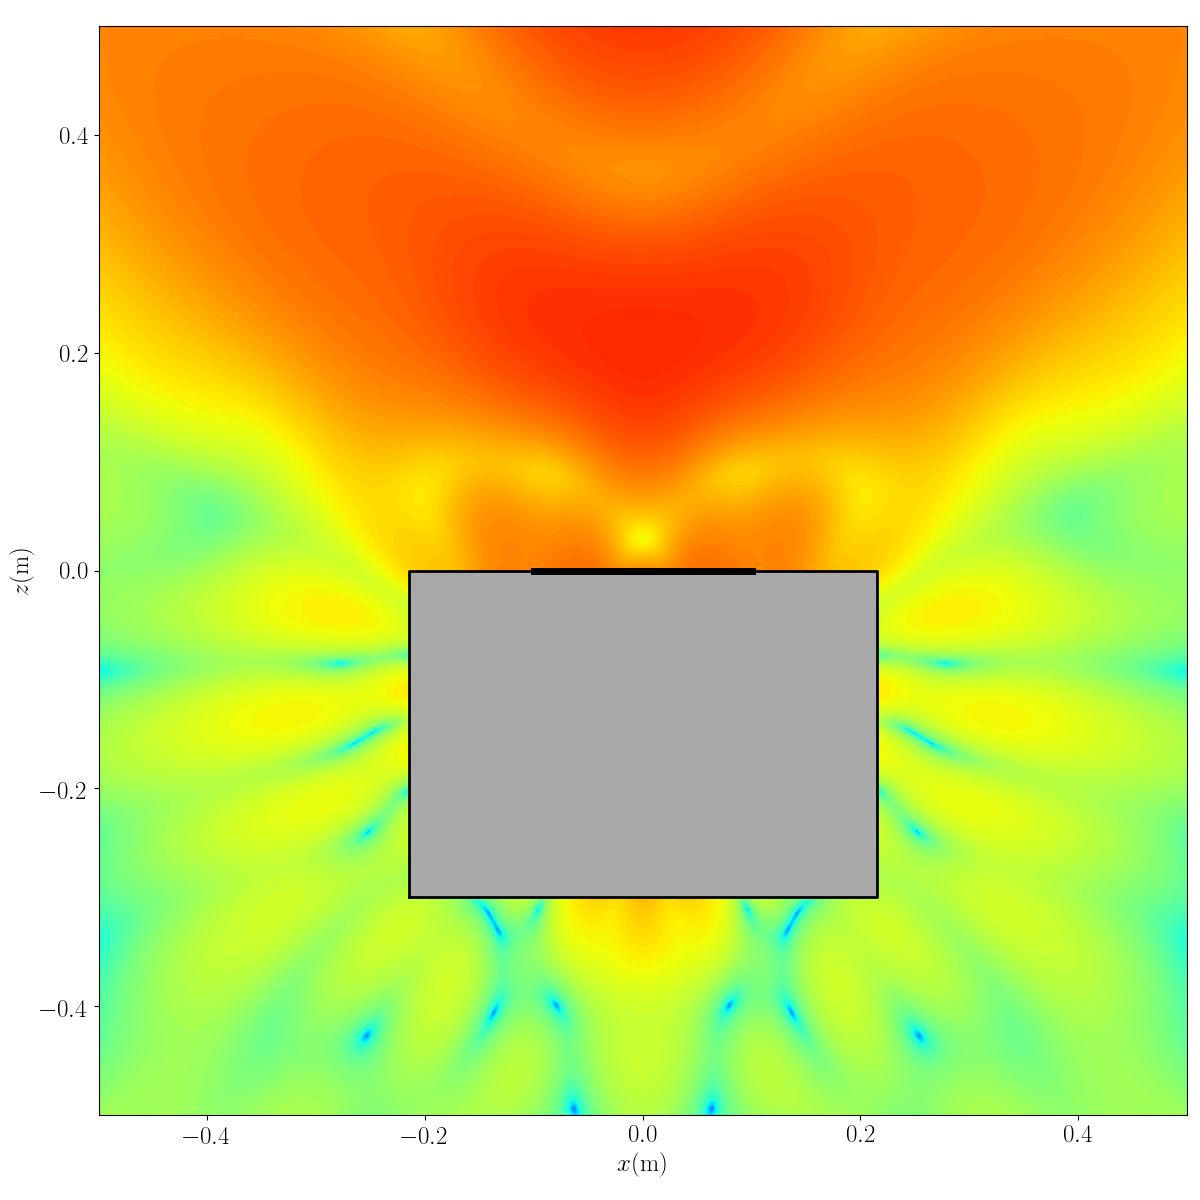
\includegraphics[width=3in]{figures/4000.png}}%
    \only<22>{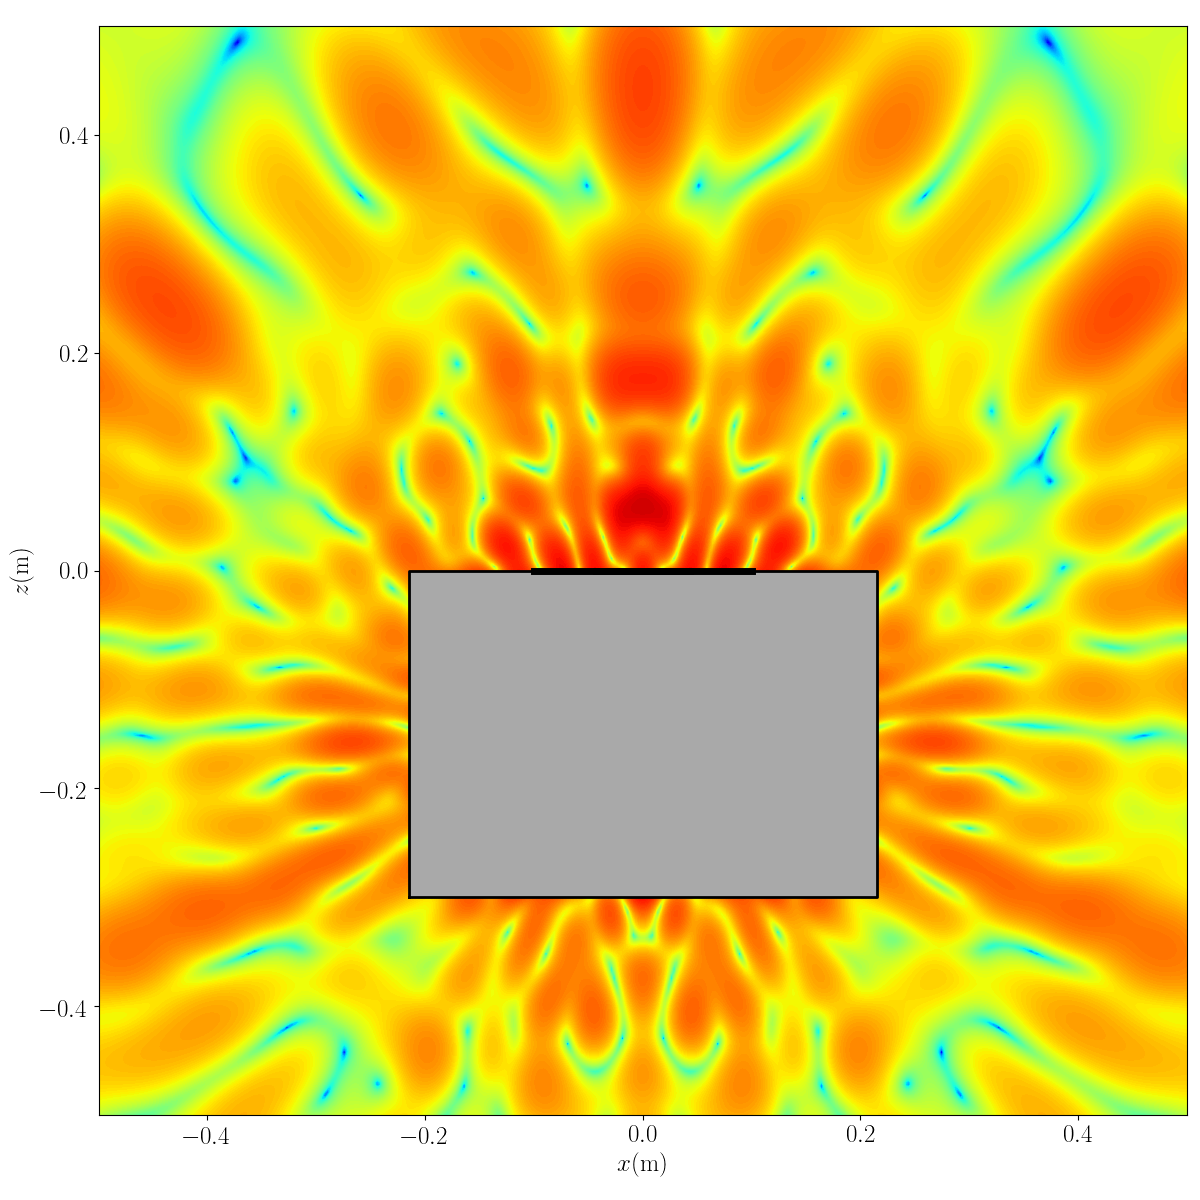
\includegraphics[width=3in]{figures/8000.png}}%
  \end{center}
\end{frame}

%------------------------------------------------------------------------

\begin{frame}
  \frametitle{Helmholtz Equation (axisymmetric 2D)\\
    \csub{\small Place equally-spaced sources just inside tweeter}}
  \begin{itemize}
  \item Simulation of loudspeaker driver on infinite baffle
  \item Construct source ring for axisymmetric problem
    \begin{align*}
      \bar{G}_j(r,z) = &~\oint \frac{d\phi}{2\pi} \, \frac{e^{i k R_j}}{4 \pi R_j} \; , \\
      R_j = &~R_j(r,r_j,z,z_j,\phi-\phi_j)
    \end{align*}
  \item Use trapezoidal integration with refinement until convergence
  \end{itemize}
\end{frame}

%------------------------------------------------------------------------

\begin{frame}
  \frametitle{Helmholtz Equation (axisymmetric 2D)\\
    \csub{\small Place equally-spaced sources just inside tweeter}}
  \begin{center}
    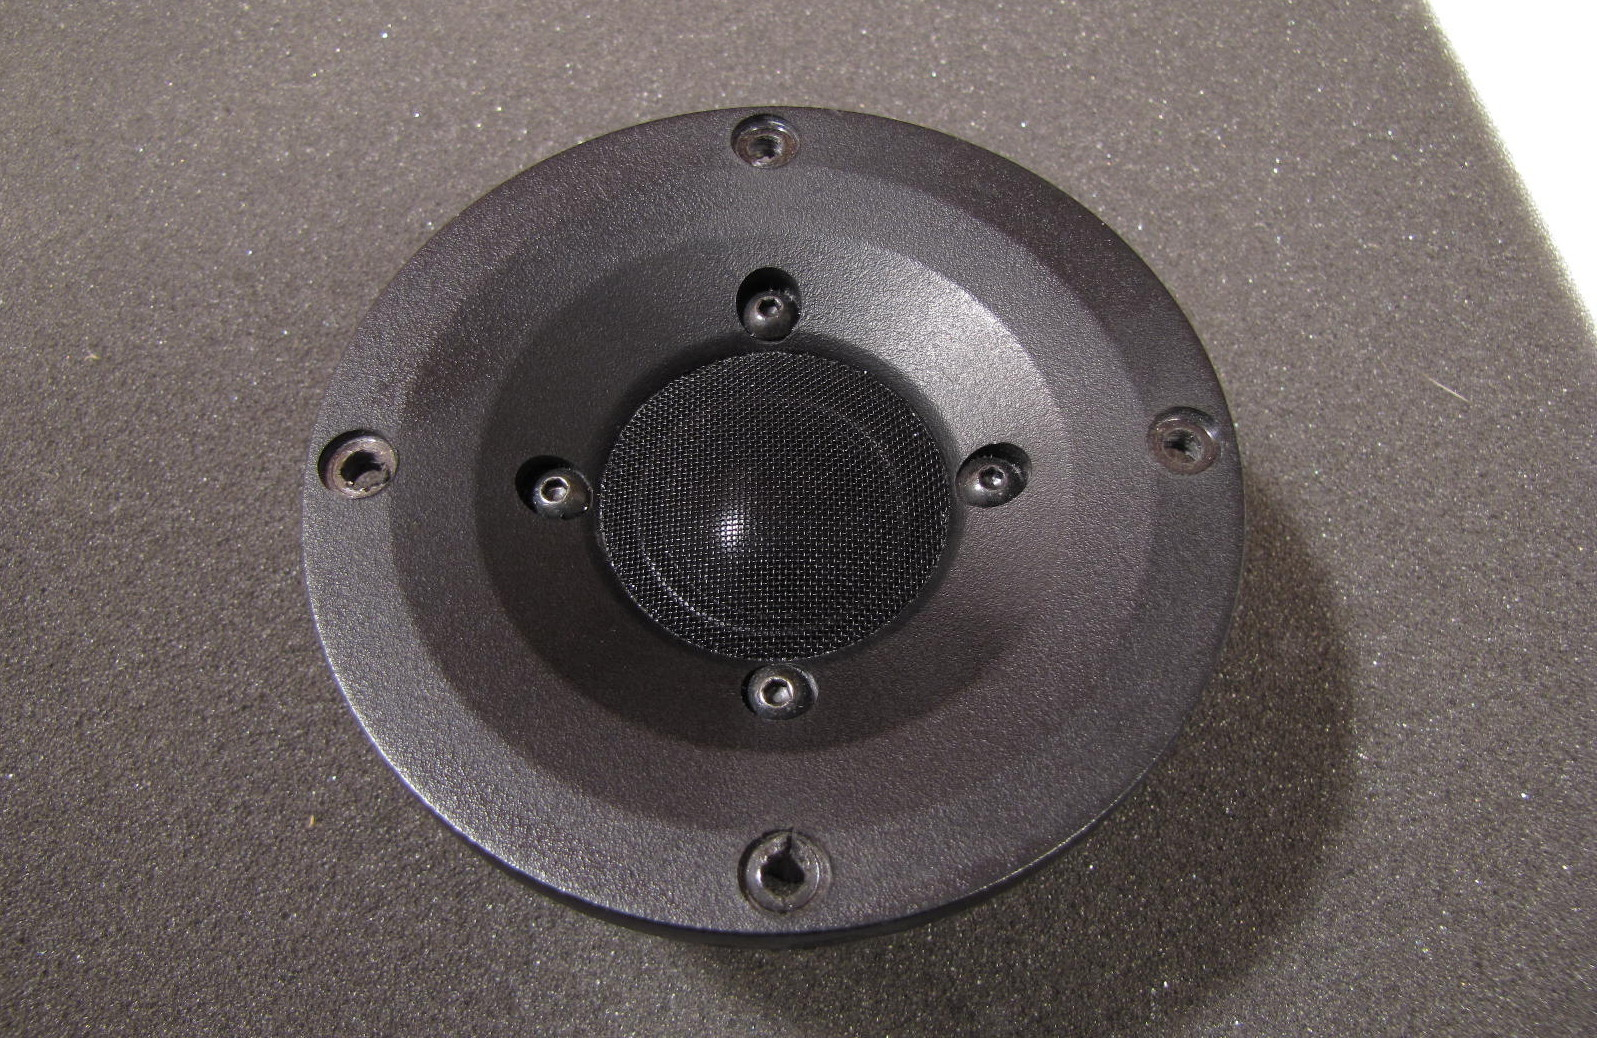
\includegraphics[width=4in]{figures/dxt_front.jpg}
  \end{center}
\end{frame}

%------------------------------------------------------------------------

\begin{frame}
  \frametitle{Helmholtz Equation (axisymmetric 2D)\\
    \csub{\small Place equally-spaced sources just inside tweeter}}
  \begin{center}
    \includegraphics[width=6.2in]{../../../../Dropbox/jaamdata/audio_work/DI/mfsa/dxt/cad.png}
  \end{center}
\end{frame}

%------------------------------------------------------------------------

\begin{frame}
  \frametitle{Helmholtz Equation (axisymmetric 2D)\\
    \csub{\small Place equally-spaced sources just inside tweeter}}
  \begin{center}
    \includegraphics[width=2.4in]{../../../../Dropbox/jaamdata/audio_work/DI/mfsa/dxt/error.png}
    \includegraphics[width=3.5in]{../../../../Dropbox/jaamdata/audio_work/DI/mfsa/dxt/polar.png}

  \end{center}
\end{frame}

%------------------------------------------------------------------------

\begin{frame}
  \frametitle{Helmholtz Equation\\
    \csub{\small Choose coefficients to satisfy BCs}}
  \begin{center}
    \vskip -3mm
    \includegraphics[width=2.4in]{../../../../Dropbox/jaamdata/audio_work/DI/mfsa/dxt/p.png}
    \includegraphics[width=2.4in]{../../../../Dropbox/jaamdata/audio_work/DI/mfsa/dxt/v.png}
  \end{center}
\end{frame}
